\chapter{Guía de solución de problemas}
\label{chapter: troubleshooting}

\section{Mensajes de error}

\subsection{Carpeta no encontrada}
El simulador arrojará el error de la figura 
\ref{fig: path error} si la carpeta \textbf{funciones}
no fue agregado al Path de MATLAB.

\textbf{Solución.} Desde la ventana de directorio actual, 
hacer clic derecho en la carpeta de funciones.
Seleccionar la opción \textbf{Add Path} y elegir \textbf{Selected Folders}.

\begin{figure}[htb!]
 \centering
 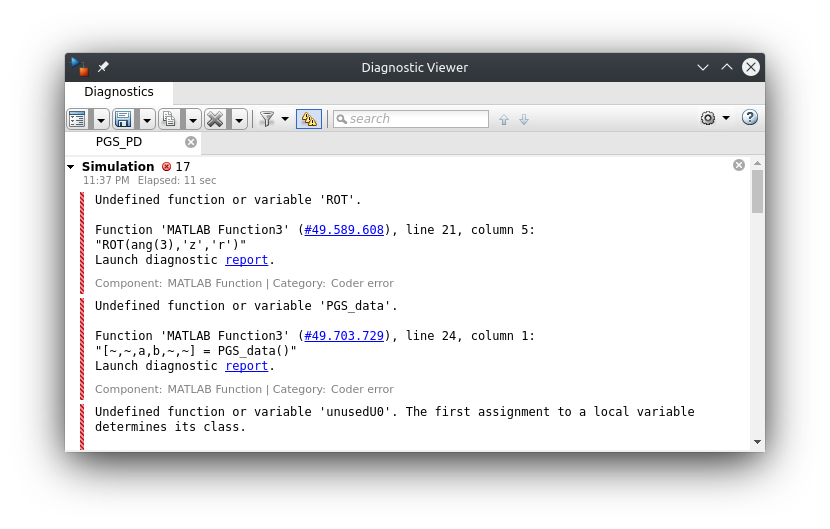
\includegraphics[scale=0.6]{error_path.png}
 \caption{Funciones no disponibles.}
 \label{fig: path error}
\end{figure}

\subsection{Esquema no ejecutable}
Este error surge por problemas de compatibilidad con otras versiones de MATLAB.

\textbf{Solución.}
Copie los bloques del esquema de control a un nuevo documento y 
replique las uniones entre bloques del esquema original.

\subsection{Errores del integrador numérico}
Ocasionado por alterar las propiedades del integrador en
los documentos. 
Se recomienda guardar una copia de seguridad 
de los archivos antes de hacer cambios.

